% !TeX spellcheck = en_GB

\PassOptionsToPackage{implicit=true}{hyperref}

\documentclass[10pt, aspectratio=1610, compress, protectframetitle, handout]{beamer}
\usefonttheme{professionalfonts}
\setbeamertemplate{blocks}[rounded][shadow=true]

\usepackage[normalem]{ulem}
\usepackage[T1]{fontenc}
\usepackage{graphicx}
\usepackage{booktabs}
\usepackage{wrapfig}
\usepackage{float}
\usepackage{datetime}
\usepackage{textpos}
\usepackage{xcolor}
\usepackage{bm}
\usepackage[ruled,vlined]{algorithm2e}
\usepackage{mathtools}
\usepackage[autostyle]{csquotes}
\usepackage[export]{adjustbox}

\MakeOuterQuote{"}

\usepackage{appendixnumberbeamer}
\usepackage[british]{babel}
\usepackage{wrapfig}
\usepackage{emoji}

\usetheme[titleformat=regular, sectionpage=progressbar, subsectionpage=none, numbering=fraction, progressbar=frametitle, block=fill]{metropolis}
\setmonofont{FiraMono-Regular.otf}

\graphicspath{{img/}}

\definecolor{MetroLinks}{RGB}{96, 76, 56}
\definecolor{MetroCite}{RGB}{35, 55, 59}
\definecolor{MetroUrl}{RGB}{20, 176, 61}

\hypersetup{
    colorlinks,
    linkcolor=MetroLinks,
    citecolor=MetroCite,
    urlcolor=MetroUrl,
}

\DeclareMathOperator*{\argmax}{arg\,max}
\DeclareMathOperator*{\argmin}{arg\,min}
\DeclareMathOperator*{\kldiv}{\text{KL}}
\newcommand{\cardof}[1]{|#1|}
\newcommand{\condon}{|}
\newcommand{\ddiff}[1]{\mathop{d#1}}
\newcommand{\dimof}[1]{\text{dim}(#1)}
\newcommand{\dpart}[1]{\mathop{\partial#1}}
\newcommand{\fullstop}{\text{ .}}
\newcommand{\mat}[1]{\bm{#1}}
\newcommand{\netw}[1]{\mathcal{#1}}
\newcommand{\normof}[1]{||#1||}
\newcommand{\suchthat}{\textit{s.t.\ }}
\newcommand{\etc}{\textit{etc.\ }}
\newcommand{\wlogg}{\textit{w.l.o.g.\ }}
\newcommand{\wrt}{\textit{w.r.t.\ }}
\renewcommand{\vec}[1]{\bm{#1}}
\newcommand{\carso}{\texttt{CARSO}\ }

% Change Colors/Width of Progress Bars
\makeatletter
\setlength{\metropolis@progressonsectionpage@linewidth}{3pt}
\makeatother

% Quoting tools
\let\oldquote\quote
\let\endoldquote\endquote
\renewenvironment{quote}[2][]
{\if\relax\detokenize{#1}\relax
    \def\quoteauthor{#2}%
    \else
    \def\quoteauthor{#2~---~#1}%
    \fi
    \oldquote}
{\par\nobreak\smallskip\hfill(\quoteauthor)%
    \endoldquote\addvspace{\bigskipamount}}


\title{\textsc{\texttt{C}ounter\texttt{A}dversarial \texttt{R}ecall of \texttt{S}ynthetic \texttt{O}bservations}}
\subtitle{A \textit{neuro-inspired} approach to foil gradient-based adversarial attacks}
\author{Emanuele \textsc{Ballarin}\inst{$\dagger$}}
\institute[]{
    \inst{$\dagger$} \scshape{\texttt{AICPS} $\in$ Dept. of Mathematics $\subseteq$ Univ. of Trieste} |
    \inst{$\ddagger$} \scshape{\texttt{AREA} Science Park}
}

\addtobeamertemplate{frametitle}{}{%
    \begin{textblock*}{100mm}(0.8\textwidth,-0.94cm)
        \hspace{10px}
        
\includegraphics[valign=c, height=0.4cm]{logo_adsai_bw_scaled}
        \hspace{3px}
        
\includegraphics[valign=c, height=0.4cm]{logo_dssc_white}
        \hspace{2px}
        
\includegraphics[valign=c, height=0.45cm]{logo_units_white}
\end{textblock*}}

\begin{document}
    % !TeX spellcheck = en_GB

\setbeamertemplate{title page}{
    \begin{minipage}[b][\paperheight]{\textwidth}
        \ifx\inserttitlegraphic\@empty\else\usebeamertemplate*{title graphic}\fi
        \vfill
        \ifx\inserttitle\@empty\else\usebeamertemplate*{title}\fi
        \ifx\insertsubtitle\@empty\else\usebeamertemplate*{subtitle}\fi
        \usebeamertemplate*{title separator}
        \vspace*{4px}
        \begin{minipage}[]{0.5\textwidth}
            \ifx\beamer@shortauthor\@empty\else\usebeamertemplate*{author}\fi
            \vspace*{1.8em}
        \end{minipage}
        \begin{minipage}[]{0.5\textwidth}
            \raggedleft
            {\small Supervised by: Prof. Luca \textsc{Bortolussi}{${}^\dagger$} \par}
            \vspace*{0.2em}
            {\small CoSupervised by: Dr. Alessio \textsc{Ansuini }{${}^\ddagger$}}
        \end{minipage}
        \vspace*{7px}
        \center\small Graduation session: M.Sc. in \textit{Data Science and Scientific Computing}
        \center\ifx\insertdate\@empty\else\usebeamertemplate*{date}\fi
        \vspace*{14px}
        \raggedright\ifx\insertinstitute\@empty\else\usebeamertemplate*{institute}\fi
        \vspace*{15px}
    \end{minipage}
}

\frame{\titlepage}

    % !TeX spellcheck = en_GB

\begin{frame}{\mbox{ }}

    \begin{center}
    \underline{An \textit{elevator pitch}}
    \end{center}

    \texttt{CARSO} (\textit{CounterAdversarial Recall of Synthetic Observations}) is a \alert{novel} \textit{deep learning} architecture and training/inference methodology for the improvement of \alert{\textit{adversarial robustness}} in \textit{deep artificial neural networks}.

    \begin{itemize}
        \item Loosely inspired by high-level \textit{neurocognitive} mechanisms;
        \item Targeted against \textit{\alert{gradient}-based}, \textit{white-box} attacks;
        \item Significant, promising results so far; comprehensive testing still in early stages.
    \end{itemize}

\end{frame}
    % !TeX spellcheck = en_GB

\begin{frame}{\protect{\emoji{thinking-face}} \textit{Deep Learning} in 2022}

\textit{Deep learning} today is a remarkably powerful and mature paradigm, able to reach (super)human-level performance in (selected) \textit{regression}, \textit{classification}, data \textit{generation} and \textit{control} tasks.

\center 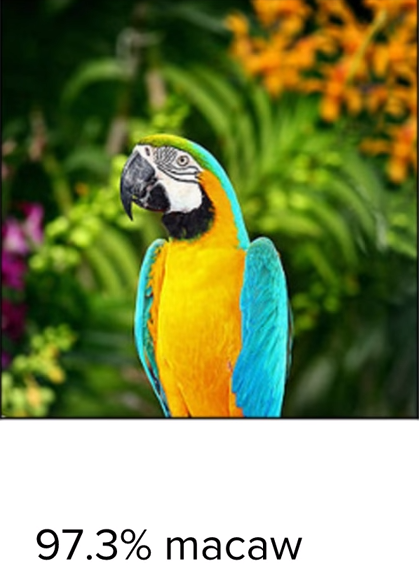
\includegraphics[height=0.35\linewidth]{macaw_macaw.png}
\end{frame}

\begin{frame}{\protect{\emoji{thinking-face}} Also \textit{Deep Learning} in 2022}

    However...

\center 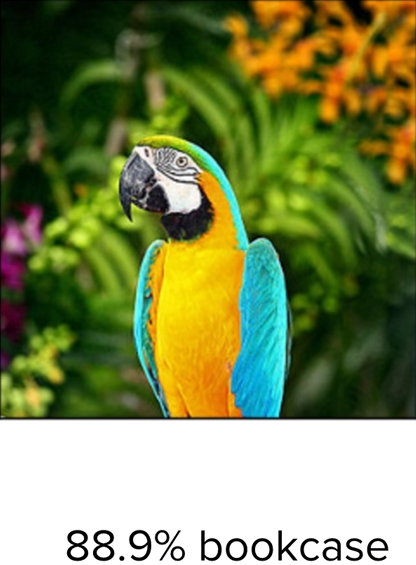
\includegraphics[height=0.35\linewidth]{macaw_bookcase.png}

\hspace*{14px}\textit{(P. Perdikaris, 2018)}
\end{frame}
\setcounter{footnote}{0}

\begin{frame}{\protect{\emoji{thinking-face}} \textit{Adversarial inputs and attacks}}
    The last shown picture is an example of
    \hfill\break
    \begin{block}{\textit{Adversarial Input}}
        An \textit{input} is said to be \textit{adversarial} to a machine learning system if it alters its \alert{reasonably} expected behaviour\footnote{Usually from the \textit{P.o.V.} of the user(s).}. Also called \textit{adversarial attack}, stressing the intentional\footnote{Which is not a strict requirement, though!} crafting of it.
    \end{block}

In the specific case of a classifier: produce a \textit{misclassification}.
\end{frame}


\begin{frame}{\protect{\emoji{thinking-face}} Why studying \textit{adversarial robustness}?}

    We live in times where a growing portion of even \textit{high-stakes} \alert{decisions} is \alert{delegated} to autonomous systems (\textit{e.g.} \textit{HR} selection, insurance, health, fraud detection, \etc\dots).

    \underline{Purely \textit{technical} reasons}
    \begin{itemize}
        \item Harden \textit{ML/DL} systems against \alert{misuse} and \textit{input-tampering};
        \item Assess (and \textit{\alert{patch}!}) behaviour where it the most fragile.
    \end{itemize}

    \underline{\textit{Legal / ethical / social} reasons}
    \begin{itemize}
        \item To ensure \alert{compliance} with regulatory frameworks or coordinated initiatives thereof;
        \item Increase understanding, transparency, and societal \alert{trust}.
    \end{itemize}

    \underline{Broader-reaching goals}
    \begin{itemize}
        \item Use \textit{robustness} as a lens through which to study \textit{\alert{neurocognitive} phenomena}.
    \end{itemize}
\end{frame}

\begin{frame}{\protect{\emoji{thinking-face}} A (more) precise definition of \textit{robustness}}

    We can always reformulate the problem of \textit{adversarial inputs} as one of \textit{\alert{adversarial perturbations}}, \textit{i.e.}
    $$ \vec{x}_{\text{adversarial}} \coloneq  \vec{x}_{\text{legitimate}} + \alert{\vec{p}}$$

    leading to the following

    \begin{block}{Definition: \textit{\alert{$\epsilon$}-perturbative adversarial attack against classifier $\netw{N}$ in $x_0 \in \mathbb{I}$, \wrt $\normof{\cdot}$}}
        Any $\vec{x^{\star}} \coloneq \vec{x_0} + \vec{p} \text{ | } \netw{N}(\vec{x^{\star}}) \neq \netw{N}(\vec{x_0})$ and $\normof{\vec{p}} < \epsilon$
    \end{block}
\end{frame}

\begin{frame}{\protect{\emoji{brain}} \textit{At the end of the day}...}

    No optimal, universal defence! Many \textit{case-by-case} results, many \textit{trade-offs}, practically no \textit{robust-by-design} applicable solution.
    \hfill\break

    \begin{block}{A remark}
        But... have \textit{\alert{you}} ever experienced an \textit{adversarial(-like) phenomenon?}
    \end{block}

\end{frame}

    % !TeX spellcheck = en_GB

\begin{frame}{\protect{\emoji{brain}} Recall, introspection... \textit{robust AI}?}

    Indeed, \textit{brains} may be the \textit{only} practical realisation of a system with the \textit{robustness} properties we look for...
    \hfill\break
    \begin{block}{\protect{\emoji{light-bulb}} A guiding idea}
        Is it possible to loosely inform the development of \textit{robust} DL systems with (grossly simplified, idealised) descriptions of \alert{neurocognitive} phenomena?
    \end{block}
    \hfill\break
    Getting inspiration from the ideas of  \textit{\alert{recall} of acquired information}, and \textit{\alert{introspection}} as \textit{thought about thought}.
\end{frame}

\begin{frame}{\protect{\emoji{brain}} A crucial remark!}
    \begin{block}{\protect{\emoji{warning}} Beware!}
        The \textit{modelling} that follows has no claim of \textit{biological plausibility} whatsoever, at this stage! This would be \textit{added value}, though -- and in interesting research direction!
    \end{block}
\end{frame}

    % !TeX spellcheck = en_GB

\begin{frame}{\protect{\emoji{robot}} Training \texttt{CARSO}}
    \begin{minipage}[]{0.5\textwidth}
        \vspace{0px}
        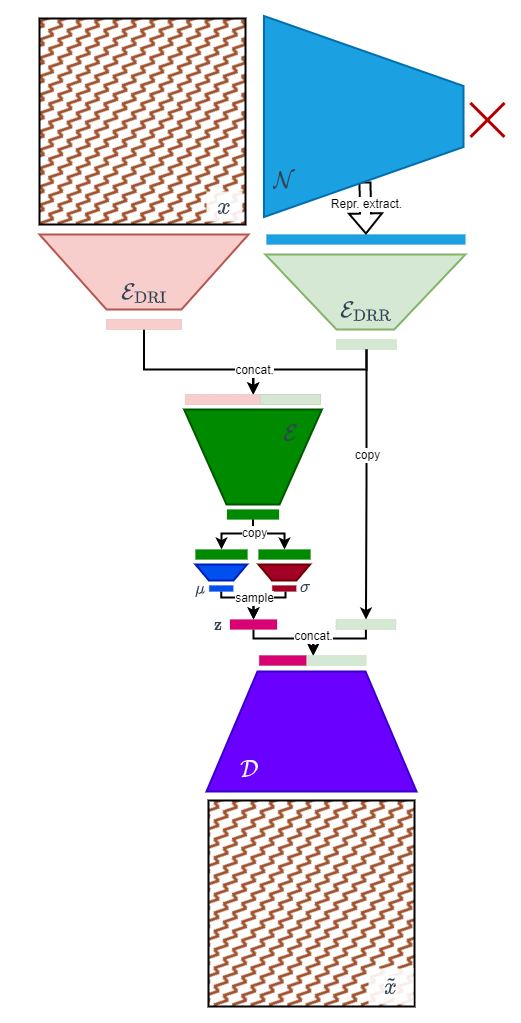
\includegraphics[width=0.91\textwidth, height=0.95\textheight, keepaspectratio]{traindiag}
    \end{minipage}
    \begin{minipage}[]{0.45\textwidth}
        \vspace{0pt}

        \begin{center}
            \underline{\textit{TL;DR:} Just a \textit{fancy \texttt{cVAE}}!}
        \end{center}

        Given an \textit{\alert{adversarially}-pretrained} classifier (for the problem of interest, and according to a given \textit{\alert{threat model}}):
        \hfill\break
        \begin{itemize}
            \item First \textit{classification pass} for representation \alert{extraction};
            \item Pre-encoding and \alert{rebalancing} of input \& representation;
            \item As in \texttt{cVAE}, aiming at \textit{\alert{purified} input} reconstruction from any input.
        \end{itemize}

    \begin{block}{Requirements}
        A dataset of \textit{clean/attacked} inputs to the classifier is needed (but \alert{no labels}!). Threat models may differ.
    \end{block}

    \end{minipage}
\end{frame}

\begin{frame}{\protect{\emoji{robot}} Inference with \texttt{CARSO}}
    \begin{minipage}[]{0.5\textwidth}
        \vspace{0px}
        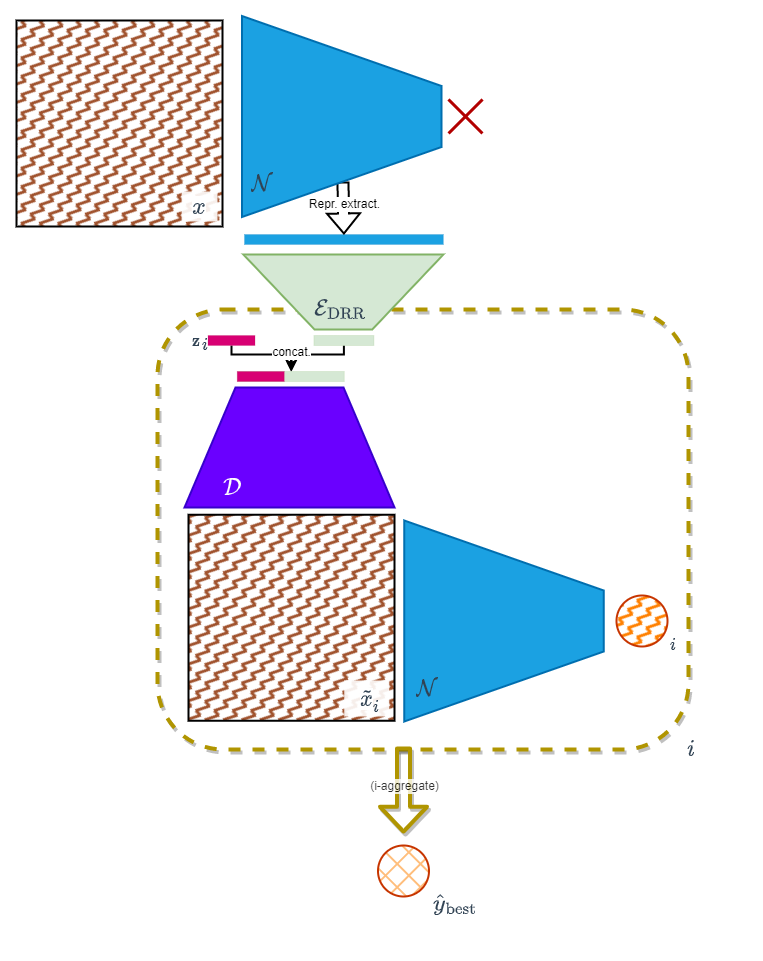
\includegraphics[width=0.95\textwidth, height=0.95\textheight, keepaspectratio]{inferdiag}
    \end{minipage}
    \begin{minipage}[]{0.45\textwidth}
\vspace{0pt}

\begin{center}
    \underline{\textit{TL;DR:} Condition, sample, classify, aggregate!}
\end{center}

Given the same \textit{adversarially-pretrained} classifier, the just-trained \textit{representation pre-compressor} and \textit{decoder}:
\hfill\break
\begin{itemize}
    \item First \textit{classification pass} for representation \alert{extraction};
    \item Representation \textit{pre-encoding};
    \item \alert{Repeated sampling} of \textit{candidate purified inputs};
    \item Second classification pass on such reconstructions, for \alert{actual classification};
    \item \alert{Aggregation} of results.
\end{itemize}
\end{minipage}
\end{frame}

    % !TeX spellcheck = en_GB
\setcounter{footnote}{0}

\begin{frame}{\protect{\emoji{test-tube}} Experimental results}
    \vspace*{11px}

    \centering
    \begin{tabular}{@{}lllll@{}}
        \toprule
        Attack / Defence (\textit{adv. acc.\%})            & None           & \texttt{IAT}   & \texttt{CARSO} &   \\
        \midrule
        None                                               & \textbf{98.40} & 97.17          & 96.72          &   \\
        \midrule
        FGSM $\normof{\cdot}_2$, $\epsilon=0.15$           & 12.09          & 91.89          & \textbf{93.62} &   \\
        FGSM $\normof{\cdot}_2$, $\epsilon=0.30$           & 01.21          & 76.94          & \textbf{86.43} &   \\
        \midrule
        (U) FGSM $\normof{\cdot}_2$, $\epsilon=0.50$       & 01.00          & 12.29          & \textbf{13.59} &   \\
        \midrule
        PGD $\normof{\cdot}_{\infty}$, $\epsilon=0.15$     & 01.60          & 90.54          & \textbf{93.44} &   \\
        PGD $\normof{\cdot}_{\infty}$, $\epsilon=0.30$     & 06.85          & 71.26          & \textbf{86.27} &   \\
        \midrule
        (U) PGD $\normof{\cdot}_{\infty}$, $\epsilon=0.50$ & \textit{20.66} & \textit{11.67} & \textbf{38.38} &   \\
        \midrule
        (U) DF $\normof{\cdot}_{\infty}$, $\epsilon=0.15$  & 00.66          & 90.25          & \textbf{95.06} &   \\
        (U) DF $\normof{\cdot}_{\infty}$, $\epsilon=0.30$  & 00.00          & 60.54          & \textbf{93.31} &   \\
        (U) DF $\normof{\cdot}_{\infty}$, $\epsilon=0.50$  & 00.00          & 00.78          & \textbf{71.34} &   \\ \bottomrule
    \end{tabular}
\end{frame}

    % !TeX spellcheck = en_GB

\begin{frame}{\protect{\emoji{speaking-head}} Discussion}

    Within the scope of the experimental analysis performed so far, we consider the results obtained to be \textit{moderately-to-very} \alert{positive}.

    \begin{itemize}
        \item A \textit{clean accuracy \alert{toll}} is imposed by the method \wrt \textit{IAT}. Yet, this is to be generally expected, and slight in magnitude;
        \item Against \underline{\textit{foreseen attacks}}: significant -- but not large -- increase in \textit{adversarial accuracy};
        \item Against \underline{\textit{unforeseen attacks}}: very solid performance, clearly beyond \textit{foreseen attacks/defences} transferability. \textit{Innate robustness}
    \end{itemize}

Speculatively: the result of a combined, synergistic effect. However, the lens of the \textit{data manifold hypothesis} may give a more precise analysis: \texttt{CARSO} acts mainly as an \textit{on manifold re-projector}!
\end{frame}
    % !TeX spellcheck = en_GB
\begin{frame}{\protect{\emoji{rocket}} Where did we came from, where do we go?}

    We talked about \texttt{CARSO} -- a novel framework devised to foil \textit{gradient-based adversarial attacks}, specifically targeted at image classification -- showing noteworthy improvements upon \texttt{IAT}, a strong contribution to \textit{off-manifold-to-on-manifold reprojection}, and solid \textit{innate robustness}.

    Experimental scope can be -- and will be! -- broadened, though, to a wider set of \textit{neural architectures}, \textit{types} of data, or more complex, challenging (classification) tasks.

\end{frame}

\begin{frame}{\protect{\emoji{rocket}} Beyond \texttt{CARSO}}

    The work required to develop and assess \texttt{CARSO} evoked suggestions reaching far longer and broader than expected. Chiefly, in order of increasing conceptual distance...

    \begin{itemize}
        \item The idea that \textit{adaptive} defences may exist, explicitly steering their behaviour on the basis of the geometric properties of inputs or attacks faced.
        \item Weight-agnostic layers operating at the \textit{feature-specific}, able to produce \textit{zero-gradient} in expectation.
        \item The possibility of informing the development of \textit{deep learning} architectures with neural activity recordings from even \textit{live-subjects}. \protect{\emoji{mouse}}
    \end{itemize}
\end{frame}

    % !TeX spellcheck = en_GB

\phantomsection
\begin{frame}{\protect{\emoji{folded-hands}}Thanks for your attention!}
    \centering
    \vspace*{25px}
    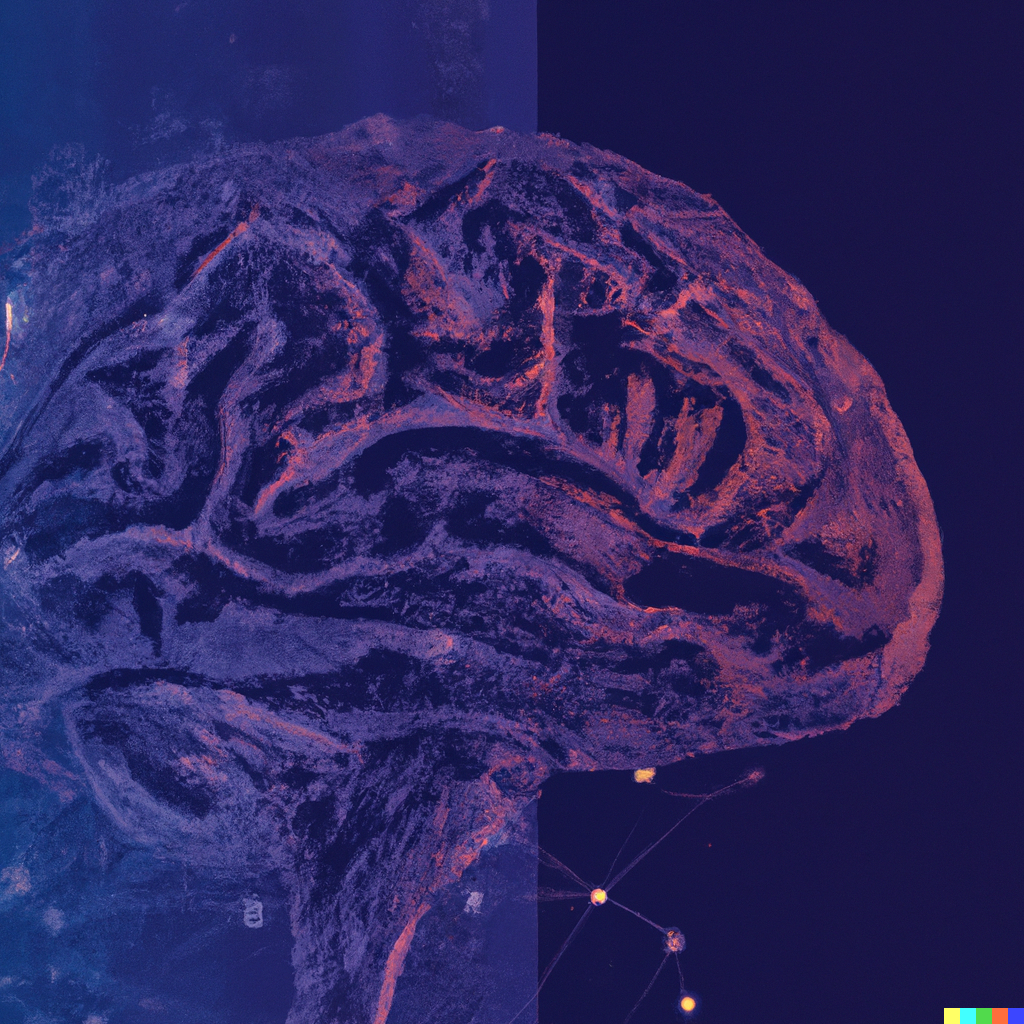
\includegraphics[width=0.9\textwidth, height=0.7\textheight, keepaspectratio]{dallecarso}
    \vspace*{10px}
\end{frame}

\end{document}
